\begin{center}{ \bf  ОБ ОТРАЖЕНИИ НА ДИНАМИЧЕСКОМ ЗЕРКАЛЕ В ОДНОРОДНОМ ПОЛЕ}\\
{\it А.Н.Токарева, А.В. Хмельницкая} \\
\end{center}
\addcontentsline{toc}{section}{Токарева А.Н., Хмельницкая А.В.\dotfill}

Развитие сверхмощных лазеров требует найти новые виды отражающих поверхностей. Статические плоские и в форме эллиптического цилиндра, сгорающие за очень короткий промежуток времени, могут быть заменены динамическими, поверхность которых состоит из движущихся частиц. Как известно, в однородном поле тяжести, когда все линии напряженности параллельны друг другу, траектория движения не вертикально падающего тела есть парабола. Таким же будет движение заряженной частицы в однородном поле заряженной плоскости, имеющий заряд противоположного знака, если начальная скорость не параллельна линиям напряженности.

Здесь представлено определение кривой, состоящей из точек отражения луча, идущего из точки S в точку $P$на семействе парабол, задаваемых формулой $y=axІ?+c$, где $a<0$, $с$-константа, определяющая конкретную кривую семейства. Как видно из формулы, вершины семейства парабол находятся на оси OY, ветви направлены вниз.

В простейшем случае точку источника S совместим с началом координат (Рис.1), а точку $P$ на оси OX, тогда известное правило отражения о равенстве падающего и отраженного угла можно формализовать в виде равенства нулю скалярного произведения

$(\overrightarrow{фo},\overrightarrow{N})=0$, в котором$\overrightarrow{N}=\frac{{\rm 1}}{|\overrightarrow{OM}|\ }\overrightarrow{OM}+\frac{{\rm 1}}{|\overrightarrow{PM}|\ }\overrightarrow{PM}$, а $\overrightarrow{\tau }=\left\{1;y'\right\}.$

Для семейства парабол $y=ax^2+c$\\
$y'=2ax$, с учётом того, что $\overrightarrow{OM}=\left\{x,y\right\},\ \overrightarrow{PM}=\left\{x-p,y\right\},$ получаем

\begin{equation} \label{GrindEQ__1_} \sqrt{x^{{\rm 2}}{\rm +}{{\rm y}}^{{\rm 2}}}\left(p-x-2axy\right)=\sqrt{(x-{p)}^{{\rm 2}}{\rm +}y^{{\rm 2}}}\left(x+2axy\right) \end{equation}

В зависимости от расположения параболы относительно точек S и $P$. Отражение может быть внутренним и внешним.

\begin{figure}
	\centering
	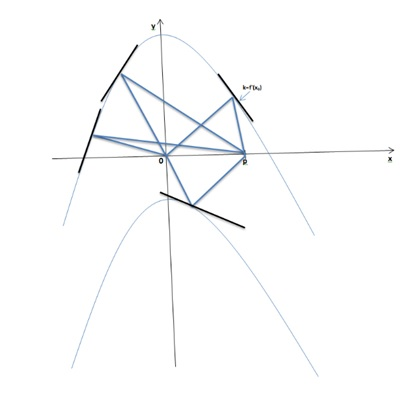
\includegraphics[width=0.9\textwidth]{tokareva1.jpg}
\end{figure}

Можно показать, что на одной параболе при нашем выборе S и $P$ точек отражения не может быть больше трех. На рисунке 1 показаны возможные точки отражения.

Мы сформулировали и рассмотрели несколько вспомогательных задач из которых следует, что на промежутке $\left(-\infty ;0\right)$каждому значению переменной $x$ соответствует единственное значение $y$ на графике исследуемой функции, причём она будет монотонно возрастать. В промежутках $\left(0;\frac{p}{2}\right)и\left(\frac{p}{2};p\right)$ прямые $x=const$ помимо значения $y=0$ могут пересекать график функции (1) ещё в одной (и это будет точка экстремума) или двух точках. На промежутке $\left(p;+\infty \right).$ наша функция также монотонно возрастает.

Наши исследования объясняют разницу в поведении графика функции (1) на участке $\left(\frac{p}{2};p\right)$.

\begin{figure}
	\centering
	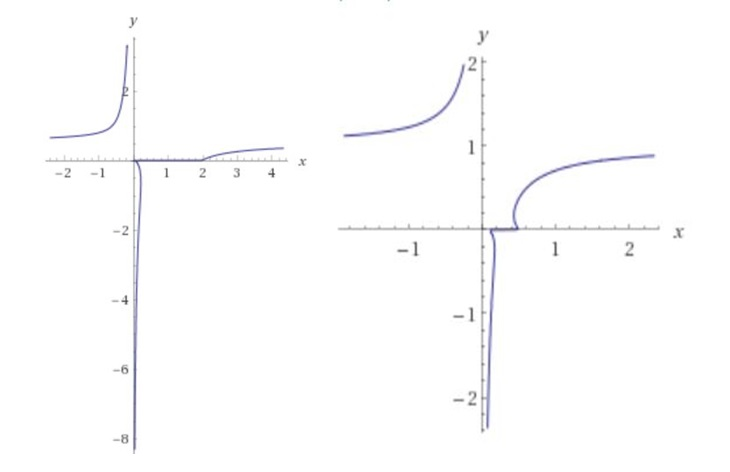
\includegraphics[width=0.9\textwidth]{tokareva2.jpg}
\end{figure}

На рисунке слева параметры: $a=-1,\ p=2$ , на рисунке справа: $a=-\frac{1}{2},\ p=\frac{1}{2}$

Установлено, что при определённых соотношениях между $a$ и $p$ можно попасть в точку $P$ из точки $S\equiv 0$ двумя способами для одного и того же $x$. Т.е. существуют две точки $M_1 $и $M_2$ на прямой $x=const\ne \frac{p}{2}$ , лежащие по одну сторону от оси $OX$, в которых отражение осуществится под разными углами $\varphi_1$ и $\varphi_2$.Найдено условие, когда $M_1=M_2$.

\begin{figure}
	\centering
	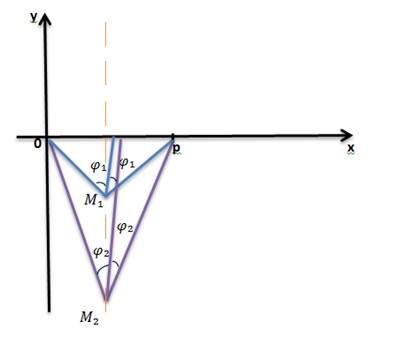
\includegraphics[width=0.9\textwidth]{tokareva3.jpg}
\end{figure}

В трёхмерном случае в условиях решаемой задачи $\overrightarrow{OM}=\left\{x,y,z\right\},\ \overrightarrow{PM}=\left\{x-p,y,z\right\}$, а вектор $\overrightarrow{\tau }=\left\{1;;2ax,0\right\}$ параллельный плоскости $OXY$, это даёт нам уравнение поверхности отражения:

\begin{equation} \label{GrindEQ__2_} \sqrt{x^2+y^2+z^2}\left(p-x-2axy\right)=\sqrt{(x-p)}^{{\rm 2}}{\rm +}y^{{\rm 2}}+z^{{\rm 2}}\ \ \left(x+2axy\right) \end{equation}

Исследование уравнения (2) проводилось методом сечения плоскостями $z=z$.

В стандартной литературе [1], [2] рассматриваются вопросы управления параметрами для достижения максимумов (минимумов) полезных функций в технически значимых прикладных задачах (потенциальной энергии, светового потока). Нами получен вид функции плоской фокусировки динамического зеркала, построенного на частицах, движущихся по параболам.

\begin{multline*}
	\rho (\varphi ,a)=
	%\\=
	K\left(1+\ tg\left(\varphi +\pi -arctg\frac{1}{2a}\right)\cdot
	\right.\\ \cdot \left.
	 ctg\left(\varphi -\pi +arctg\frac{1}{2a}\right)\right),
\end{multline*}
где  $\varphi $ -- угол падения и отражения, $K$ -- константа, определяемая значением $p$, $a$-- старший коэффициент параболы, параметр, регулируемый скоростью частиц и напряжённостью  однородного поля. Одним из применений может быть фокусировка сверхмощного лазерного излучения при помощи динамического зеркала для исследований по управляемому термоядерному синтезу.



\smallskip \centerline{\bf Литература}\nopagebreak

1. {\it Арнольд В.И.} Теория катастроф -- Москва: Изд-во «Наука», 1990.

2. {\it Брус Дж.,Джиблин П.} Кривые и особенности -- Москва: Изд-во «Мир», 1988.


